
\begin{theo} $f∈C^0_0(ℝ^2),\ 0<δ\leq\frac12$. Then
	\[∫_{S^1}R_δ^*(f)(γ)\mdσ_γ\leq\sim(\log\frac1δ)^{\frac12}(\|f\|_{L^1(ℝ^2)}+\|f\|_{L^2(ℝ^2)})\]%(*)
\end{theo}

\begin{proof}[Proof of Theorem]
	Modified version of lemma 3: Setting
	\[F_δ(t)=∫_{-∞}^∞\hat F(λ)(\frac{e^{2πi(t+δ)λ}-e^{2πi(t-δ)λ}}{2πiλ(2δ)})\mdλ\]
	Suppose $\sup_{λ∈ℝ}|\hat F(λ)|\leq A$ and $∫_{-∞}^∞|\hat F(λ)|^2|λ|^{d-1}\mdλ\leq B^2$.

	Claim:\[\sup_t|F_δ(t)|\leq\sim(\log\frac1δ)^{\frac12}(A+B)\]
	\[F_δ(t)=∫_{-∞}∞=∫_{|λ|\leq1}+∫_{|λ|>1}\leq cA+∫_{1<|λ|\leq\frac1δ}|\hat F(λ)|\mdλ+\frac cδ∫_{|λ|>\frac1δ}|\hat F(λ)||λ|^{-1}\mdλ=I+II\]
	CS: \[I\leq\sim(∫_ℝ|\hat F(λ)|^2|λ|\mdλ)^{\frac12}(∫_{1<|λ|\leq\frac1δ}|λ|^{-1}\mdλ)^{\frac12}\leq B(\log\frac1δ)^{\frac12}\]
	\[II\leq\sim\frac cδ(∫_{ℝ^2}|\hat F(λ)|^2|λ|\mdλ)^{\frac12}(∫_{|λ|>\frac1δ}|λ|^{-3}\mdλ)^{\frac12}\leq\sim B\]
\end{proof}

\begin{theo} %1
	There exists a subset $K⊂ℝ^2$ such that
	\begin{enumerate}
		\item $K$ is compact
		\item $K$ has Lebesgue measure zero
		\item $K$ contains a transatle of every unit line segment
	\end{enumerate}
\end{theo}
\begin{theo}%2
	Suppose $F$ is any set that satisfis cnditions (i) and (iii) from Theorem 1. Then $F$ has Hausdorff dimension 2.
\end{theo}
\begin{proof}[Proof of Theorem 2]
	Let $F$ be a Kakeya set. Fix $0<α<2$. Lett $F⊂\bigcup_{i=1}^∞B_i$ be a covering with balls $B_i$ of diameter $\leqδ$. It is enough to show
	\[\sum(\diam B_i)^α\geq c_α>0\]
	Case 1: Assume $\diam B_1=δ\leq\frac12$ and let $N<∞$ be the number of balls in the covering. WTS $Nδ^α\geq c_α$. $B_i^*=$ doubel of $B_i$. $F^*=\bigcup_iB_i^*$. $|F^*|\leq\sum|B_i^*|=cNδ^2$. $F$ Kakeya $⇒∀γ∈S^1∃s_γ\perpγ$ unit lime segment: $s_γ⊂F$. $s_γ^δ⊂F^*$. $\therefore R_δ^*(χ_{F^*})(γ)\geq 1\ (∀γ∈S^1)$. Take $f=χ_{F^*}$ in (*). Since $L^2⊂L^1$,
	\[\|χ_{F^*}\|_{L^1}\sim\leq\|χ_{F^*}\|_{L^2}=|F^*|^{\frac12}\sim\leq N^{\frac12}δ.\] (*) $⇒0<c\leq(\log\frac1δ)^{\frac12}N^{\frac12}δ$. This implies $Nδ^α\geq c_α>0$.

	Case 2: General case. $F⊂\bigcup_{i=1}^∞B_i$ with each ball $B_i$ of diameter $\leq 1$. For each $k∈ℕ$, let $N_k$ be the number of balls ön $\{B_i\}$ with diameter $B_k\sim 2^{-k}$, i.e.\ $∈[2^{-k-1},2^{-k}]$. WTS
	\[\sum_{k=0}^∞N_k2^{-kα}\geq c_α>0.\]
	ETS $∃K':N_{k'}2^{-k'α}\geq c_α$.
	\[F_k=F∩(\bigcup_{\diam B_i\sim 2^{-k}}B_i)\]
	\[F_k^*=\bigcup_{\diam B_v\sim 2^{-k}}B_i^*\]
	\[|F_k^*|\leq cN_k2^{-2k}\quad∀k\]
	$F$ Kakeya $⇒∀γ∈O^2∃s_γ\perpγ:s_γ⊂F$ (in particular $m_1(s_γ∩F)=1$).%(**)
	
	Key: For some $k$, a large proportion of $s_γ$ belongs to $F_k$. Pick $\{a_k\}_{k=0}^∞$ such that $0\leq a_k<1,\ \sum a_k=1,\ (a_k)$ dos not nend to 0 too quickly, e.g.\ $a_k=c_ε2^{-kε}$ (for sufficiently small $ε$.

	Claim: \[∃k:m_1(s_γ∩F_k)\geq a_k.\] Otherwise $m_1(s_γ∩F)\leq\sum_km_1(s_γ∩F_k)<\sum a_k=1$, contradicts (**)

	For this value of $k$, \[R_{2^{-k}}^*(χ_{F_k^*})(γ)\geq a_k.\]
	Since this choice of $k$ depends on $γ$, let \[E_k=\{γ∈S^1:R_{2^{-k}}^*(χ_{F_k^*})(γ)\geq a_k\}.\] $S^1=\bigcup_{k_1}^∞E_k$. Therefore $∃k':|E_{k'}|\geq2πa_{k'}$. 
	\[2πa_{k'}^2=2πa_{k'}a_{k'}\leq∫_{E_{k'}}a_{k'}\mdσ\leq_{S^1}R_{2^{-k'}}^*(χ_{F_{k'}^*})(γ)\mdσ_γ\]
	\[2^{-2k^ε}\sim a_{k'}^2\leq c(\log2^{k'})^{\frac12}|F_{k'}^*|^{\frac12}\leq c(\log 2^{k'})^{\frac12}N_{k'}^{\frac12}2^{-k'}\]
	$⇒N_{k'}2^{-αk'}\geq c_α$, provided $4ε<2-α$.
\end{proof}
\paragraph{Construction of a Kakeya set I} (Stein-Shakarch, III)

Thinner Cantor set, always taking away the half.

Take two of them, $E_0,E_1$, where $E_1$ has twice the length. Put $E_0$ on $y=1$ and $E_1$ on $y=0$. Let $F$ be the union of all line segments that join a point in $E_0$ with one in $E_1$.

\paragraph{Construction of an $ε$-Kakeya set} (Stein)


\begin{theo} Given $ε>0,\ ∃N=N_ε$ and $2^N$ rectangles $R_1,…,R_{2^N}$ wth sidelengths $1\times 2^{-N}$ sucht that
	\begin{enumerate}
		\item \[|\bigcup_{j=1}^{2^N}R_j|<ε\]
		\item the reaches $\tilde R_j$ are mutually disjoint \[|\bigcup_{j=1}^{2^N}\tilde R_j|=1\]
	\end{enumerate}
\end{theo}
\begin{proof}
	Fix $α∈(\frac12,1)$. Symmetric triangle $ABC$ with $M$ opposite $C$. Push the right part into the left part call resulting image $Φ(T)$. It constists of heart $Φ_h(T)$ and arms $Φ_a(T)$. Then
	\[|Φ_h(T)|=α^2|T|\]
	\[|Φ_a(T)|=2(1-α)^2|T|\]
	Conclusion
	\[|Φ(T)|=(α^2+2(1-α)^2)|T|\]
	$n$-fold iteration (Peron trees): Split not into two but $2^n$ parts and do everything pairwise. Key: right side of $Φ_h(A_0A_2C)$ // left side of $Φ_n(A_2A_4C)$ // $CA_2$

	Then look at heart/arms again. $|\text{arms of }Ψ_1(ABC)|\leq2(1-α)^2|T|$. $|\text{heart of }Ψ_1(ABC)|=α^2|T|\therefore|Ψ_1(ABC)|=(α^2+2(1-α)^2)|T|$.

	Iterate: Carry out this process on the heart of $Ψ_1(ABC)$ with ne replaced by $n-1$, given are the union of $2^{n-1}$ triangles.
	
	Then retranslate all $2^n$ original triangles to obtain figure $Ψ_2(ABC)$.
	\[|\text{heart of }Ψ_2(ABC)=α^2α^2|T|\]
	\[|\text{addition arms of }Ψ_2(ABC)|\leq2(1-α)^2α^2|T|\]
	\[|Ψ_n(ABC)|\leq(α^{2n}+2(1-α)^2+2(1-α)^2α^2+…+2(1-α)^2α^{2n-2})\leqα^{2n}+2(1-α)^2+\underbrace{\sum_{n=0}^∞α^{2n}}\leqα^{2n}+2(1-α)\]

\begin{figure}[H]
	\centering
	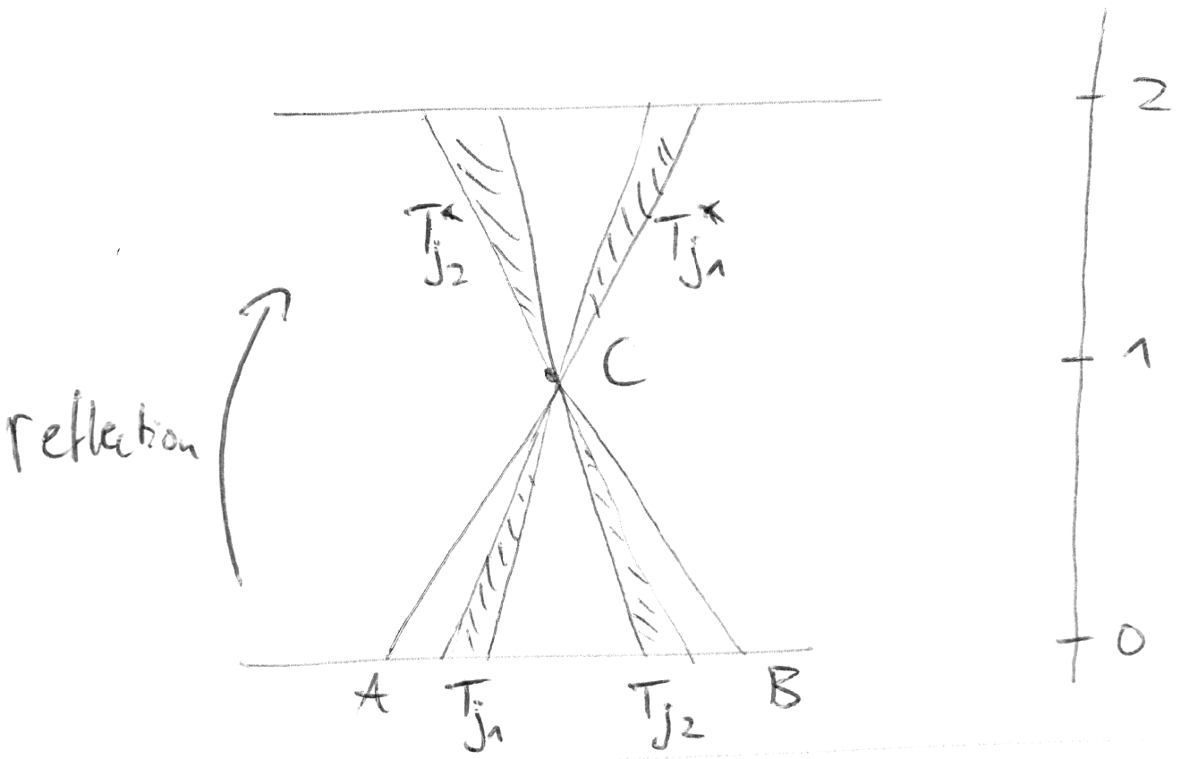
\includegraphics[height=5cm]{lec08_01}
	\caption{Obtaining mutually disjoint reaches by reflecting in $C$.}
\end{figure}

\begin{figure}[H]
	\centering
	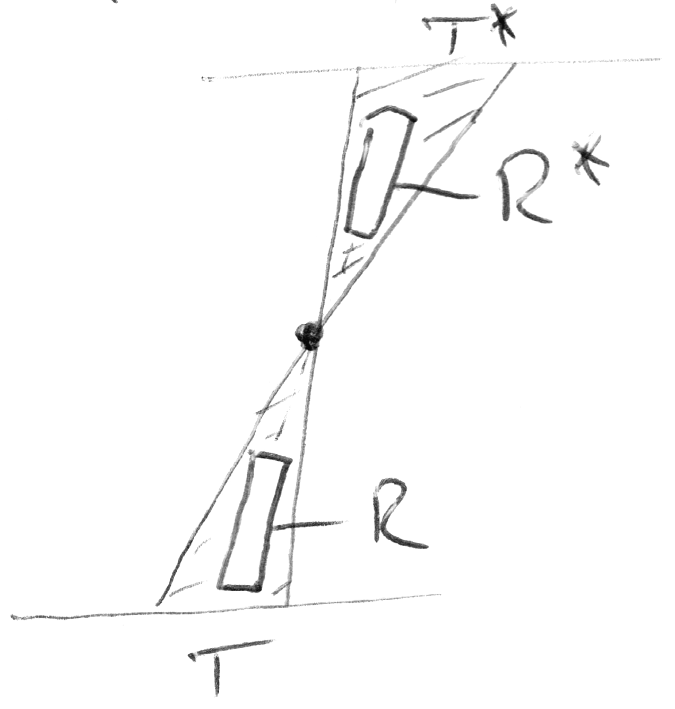
\includegraphics[height=5cm]{lec08_02}
	\caption{Go from triangles to rectangles by placing rectangles into the triangles with half the length.}
\end{figure}

\end{proof}
